
%% -- Stand: 2023/02/01
%% -- Master-Datei für die Erstellung des Beitrags 
%% -- Wir nutzen KOMA-Script
%% --
\documentclass[%
	,ngerman					% Deutsch als Standard, andere über babel
	,bibliography 	= leveldown % kein eigenes Kapitel sondern ein Abschnitt
%	,parskip = half+			% halbe Leerzeile Abstand für Absätze
	]{scrbook}

%% -- KOMA Otions
%% -- 
\KOMAoptions{%
	,paper 		= a4
	,pagesize
	,BCOR		= 15mm		% siehe KOMA-Script 2.6, S. 39
	,twoside	= true		% siehe KOMA-Script 2.6, S. 47
	,fontsize	= 12pt		% Standard ist 11pt
% 	,DIV		= calc		% siehe KOMA-Script 2.6, S. 42
	,open		= any		% siehe KOMA-Script 3.16, S. 111
	,headings 	= small		% siehe KOMA-Script 3.16, S. 113
	,open		= any
	}

%% -- Unterstützung von Paketen
%% --
\usepackage{scrhack}

%% -- Gehe davon aus, dass alle UTF8-nutzen
%% --
\usepackage[T1]{fontenc}		%% für LuaLaTeX entbehrlich


%% -- Sprache und Anführungsszeichen richtig
%% -- Andere Sprache via \selectlanguage{sprache}; siehe Manual
%% -- 
\usepackage[%
	,english
	,italian
	,french
	,main=ngerman]{babel} 

%% -- Richtige Trennung
%% --
\babelprovide[hyphenrules=ngerman-x-latest]{ngerman}

%% -- Hochkomma: Eingabe mittels \enquote{text}; dann wird alles richtig
%% --
\usepackage[%
	,autostyle
	,italian = guillemets
	,french  = guillemets
	,german  = guillemets
	,english = american]{csquotes}

%% -- Die Schrift
%% --
\usepackage{libertinus}

%% -- Das Layout
%% --
%% -- Rombuch Layout
%% -- Stand 2022/12/30
%% --

%% -- Alles etwas kleiner
%% --
\setkomafont{chapter}{\LARGE}
\setkomafont{section}{\large}
\setkomafont{subsection}{\normalsize}

%% -- Keine section etc. im TOC
%% --
\addtocounter{tocdepth}{-2}% Keine \section im TOC

%% -- chapter
%% --
%\addtokomafont{chapterentrypagenumber}{\color{white}}
\renewcommand*{\chapterformat}
 {\chapappifchapterprefix{\ }\thechapter\autodot\enskip}

\renewcommand*\raggedchapter{\centering}	% KOMA: Kapitelüberschriften zentrieren
	%
\RedeclareSectionCommand[%
  ,beforeskip	= -1.5\baselineskip
  ,afterskip		= 2.5\baselineskip
  ,innerskip		= 0.75ex
  ,tocnumwidth	= 7em
]{chapter}
%
\renewcommand*{\addchaptertocentry}[2]{%  Seite 584 / http://www.komascript.de/node/1780
  \ifstr{#1}{}{% keine Nummer:
    \addtocentrydefault{chapter}{#1}{#2}% wie bisher
  }{% mit Nummer:
    \addtocentrydefault{chapter}{}{#2} %\chapapp\ #1.-
  }%
}
%% -- Lange Zeilen zulasssen
%% -- KOMA-Script 15.3. 
%% --
\DeclareTOCStyleEntry{tocline}{chapter}

%% -- section
%% --
\renewcommand*{\thesection}{\arabic{section}} 

\RedeclareSectionCommand[tocnumwidth=2em]{section} % TOC
\renewcommand*{\addsectiontocentry}[2]{% Eintrag in TOC
  \addtocontents{toc}{\protect\addvspace{\protect.5\baselineskip}}% Halbe LZ
  \Ifstr{#1}{}{%
    \addtocentrydefault{section}{#1}{#2}%
  }{%
    \addtocentrydefault{section}{#1.}{\itshape #2}
  }%
}

%% -- subsection
%% --
\renewcommand*{\thesubsection}{\arabic{subsection}}
\renewcommand*{\subsectionformat}{\thesubsection.\enskip}% KOMA: Nummer in der Überschrift
\RedeclareSectionCommand[%
  ,beforeskip	= -1.75\baselineskip
  ,afterskip		= 0.25\baselineskip
  ,font			= \itshape
  ,tocnumwidth	= 1em
]{subsection}
%% -- Eintrag in das TOC
\renewcommand*{\addsubsectiontocentry}[2]{%
  \Ifstr{#1}{}{%
    \addtocentrydefault{subsection}{#1}{#2}%
  }{%
    \addtocentrydefault{subsection}{#1.}{#2}% Mit Punkt hinter der Nummer in TOC
  }%
}

%% -- \subsubsection: Nur Nummer 1. etc; i.a. keine Überschrift sondern es 
%% -- geht mit dem Text weiter. 
%% -- Wer es ohne die Nummer will, aber mit einer Überschrift, dann die 
%% -- Sternvariante \subsubsection*{} nutzen. 
%% -- Siehe hierzu das Musterfile für Beispiele
%% --
\setcounter{secnumdepth}{\subsubsectionnumdepth} 	% subsub-nummer
\renewcommand*{\thesubsubsection}{\arabic{subsubsection}.\kern3pt} % 1.
\RedeclareSectionCommand[%
  	,beforeskip	=  	.25\baselineskip	% Skip vor dem Kommando + indent
	,afterskip	= 	-0.1em				% Kein Skip aber Abstand
	,font		=	\normalfont			% Falls Überschrift 
%	,tocnumwidth=	1.25em				% Eintrag in TOC ist aber unterbunden
%	,tocindent	= 1em					%  
	]{subsubsection} 
	
%% -- Kopf- und Fußzeile
%% --
\RequirePackage[automark]{scrlayer-scrpage}

\clearpairofpagestyles
\renewcommand*{\chapterpagestyle}{empty}						% Nichts auf der Seite mit Kapitel

%% -- Kopfzeile
%% --
\KOMAoptions{headsepline=0.8pt}
\renewcommand*{\sectionmarkformat}{}		% keine Abschnittsnummer
\renewcommand*{\subsectionmarkformat}{}	% keine UnterAbschnittsnummer

%% ---------------------------
%% Zweiseitig
%% --------------------------
\manualmark
\ihead{\headmark} 	%% -- innen

\rohead{%% außen gerade
  \makebox[0pt][l]{%
    \makebox[\marginparsep][r]{%
      \rule[-\dp\strutbox]{1pt}{\normalbaselineskip}\nobreakspace
    }%
    \makebox[\marginparwidth][l]{\pagemark}%
  }}

\lehead{%% außen ungerade
  \makebox[0pt][r]{%
    \makebox[\marginparwidth][r]{\pagemark}%
    \makebox[\marginparsep][l]{%
      \nobreakspace\rule[-\dp\strutbox]{1pt}{\normalbaselineskip}%
    }}}

\pagestyle{scrheadings}


%% --Fußnoten Nach KOMA 3.14 
%% --
\RequirePackage[newcommands,footnotes,raggedrightboxes]{ragged2e}
\deffootnotemark{\kern1pt(\raisebox{0.35ex}{\footnotesize\thefootnotemark})}
\deffootnote[1.5em]{1em}{2em}{(\raisebox{0.35ex}{\footnotesize\thefootnotemark})\kern5pt}
\let\raggedfootnote\RaggedRight
%% %%%%%%%%%%%%%%%%%%%%%%%%%%%%%%%%%%%



%% -- Die Pakete
%% --
%% -- Die Pakete für RomSeminar
%% -- Stand: 2023/02/02
%% -- Literatur: H. Voss, Einführung in LaTeX (7. Auflage) 2022 
%% -- Muss mal sehen, wie ich dieses besser machen kann
%% --




%% -- Aufzählungen
%% -- 
\usepackage[%
	,inline			% für Aufzählungen im Text = Sternvariante
	,shortlabels	% damit \begin{enumerate}[(i)] funktioniert
	]{enumitem}
	
%% -- tikz
\usepackage{tikz}
\usetikzlibrary{positioning,arrows}

%% -- Pakete mit Referenz
%% -- 
\usepackage[newcommands,footnotes,raggedrightboxes]{ragged2e}
	
\usepackage{% Voss, LaTeX - 6.3 - Seite 227ff					
	,array 			   	
	,booktabs
	,tabularx
	,wrapfig
	,longtable}
	
\RequirePackage{% Voss, LaTeX - 8.6 - Seite 340ff					
	,caption 			   	
	,floatrow
	,subcaption}

\RequirePackage{% 						
	,multicol	% Voss, LaTeX - 5.15.1 - Seite 215	
	,parallel	% Voss, LaTeX - 5.15.2 - Seite 216
	}
	 	   	
\RequirePackage{%
	,graphicx	% Voss, LaTeX - 5.10.2 - Seite 174
	,wrapfig	% Voss, LaTeX - 5.10.3 - Seite 177
	,cutwin		% Voss, LaTeX - 5.10.3 - Seite 178
	}

%% -- Wenn schon, dann muss man es auch definieren
%% -- 
\usepackage{nicefrac}

%% -- Zum Testen
%% -- 
\usepackage{blindtext,lipsum}

%% -- Für Rahmen
%% -- 
\usepackage{mdframed}
%% -- infobox
\newmdenv{infobox} %% \begin{infobox} .. \end{infobox}





%% -- Die Abkürzungen
%% --
%% -- Richtige Interpunktion
%% --
\usepackage{xspace}
%%
%% -- Richtige Abkürzungen
% --> Englisch
\newcommand{\eg}{e.g.\xspace}
\newcommand{\ie}{i.e.\xspace}
% weitere hier eintragen

% --> Deutsch
\newcommand{\zB}{\mbox{z.\,B.}\xspace}
\newcommand{\iA}{\mbox{i.\,A.}\xspace}
\newcommand{\iAllg}{\mbox{i.\,Allg.}\xspace}
\newcommand{\di}{\mbox{d.\,i.}\xspace}
\renewcommand{\dh}{\mbox{d.\,h.}\xspace}
\newcommand{\oae}{\mbox{o.\,Ä.}\xspace}
\newcommand{\uae}{\mbox{u.\,Ä.}\xspace}
\renewcommand{\og}{\mbox{o.\,g.}\xspace}
\newcommand{\ua}{\mbox{u.\,a.}\xspace} 
\newcommand{\lc}{\mbox{l.\,c.}\xspace} 
\newcommand{\fue}{\mbox{f.\,ü.}\xspace}
%%
\newcommand{\inkl}{inkl.\xspace} 
\newcommand{\sog}{sog.\xspace} 
\newcommand{\bzgl}{bzgl.\xspace} 
\newcommand{\vs}{vs.\xspace} 
\newcommand{\ca}{ca.\xspace}
\newcommand{\bzw}{bzw.\xspace}
\newcommand{\etc}{etc.\xspace}
\newcommand{\usw}{usw.\xspace}
\newcommand{\ggf}{ggf.\xspace}
\newcommand{\evtl}{evtl.\xspace}
\newcommand{\oBdA}{o.B.d.A.\xspace}



%% --

%% -- Literatur
%% -- Die einzelnen Referenzen kann man dann mit den Möglichkeiten des Pakets lokal halten
%% -- \begin{refsection} .. \printbibliography \end{refsection} in dem jeweiligen Artikel
%% --
%% %%%%%%%%%%%%%%%%%%%%%%%%%%%%%%%%%%%%
%% Stand: 2022/10/31
%% -- Makros für biblatex
%% -- Rom-BibLaTeX.sty
%% Stand: 2023/02/07
%% %%%%%%%%%%%%%%%%%%%%%%%%%%%%%%%%%%%%
\NeedsTeXFormat{LaTeX2e}	%
\ProvidesPackage{Rom-BibLaTeX}
%% %%%%%%%%%%%%%%%%%%%%%%%%%%%%%%%%%%%%
\RequirePackage[%
  	,style 		= numeric	
   	,sorting		= nyt
	,hyperref	= true  
 	,maxnames	= 4
   	,minnames	= 3
   	,giveninits	= true		% Vornamen als Initiale Ulrich -> U.
	,backend		= biber
 	,uniquename	= false
]{biblatex}  	
%%
\ExecuteBibliographyOptions{%
 	,url		= true		% true: URL werden angezeigt
 	,doi		= false		% DOI werden im Titel hinterlegt 
	,eprint		= false		% true  - ” -
	}
%% --
%% --
\AtEveryBibitem{\clearfield{issn}}%
\AtEveryBibitem{\clearlist{language}}%
\AtEveryBibitem{\clearlist{location}}%
\AtEveryBibitem{\clearfield{pagetotal}}%
\AtEveryBibitem{\clearfield{month}}%
%% %%%%%%%%%%%%%%%%%%%%%%%%%%%%%%%%%%%%%%%%%%%%%%%%%%%%%
%% Kein Komma nach Verlag bei Büchern
%% %%%%%%%%%%%%%%%%%%%%%%%%%%%%%%%%%%%%%%%%%%%%%%%%%%%%%
\renewbibmacro*{publisher+location+date}{%
  \printlist{publisher}%
  \setunit*{\addspace}%
%  \printlist{location}%
%  \setunit*{\addsemicolon\space}%
  \usebibmacro{date}%
  \newunit%
	} % ende makro
%% %%%%%%%%%%%%%%%%%%%%%%%%%%%%%%%%%%%%%%%%%%%%%%%%%%%%%
%% Ausgabe Journal-Band(Nummer)-Jahr-Seiten
%% %%%%%%%%%%%%%%%%%%%%%%%%%%%%%%%%%%%%%%%%%%%%%%%%%%%%%	
\renewbibmacro*{journal+issuetitle}{% 
  \usebibmacro{journal}% 
  \setunit*{\addspace}% 
  \iffieldundef{series} 
    {} 
    {\newunit 
     \printfield{series}% 
     \setunit{\addspace}}% 
  \printfield{volume}% 
  \iffieldundef{number} 
     {} 
      {\kern1pt\mkbibparens{\printfield{number}}}% \addspace
  \setunit{\addcomma\space}% 
  \printfield{eid}% 
  \setunit{\addspace}% 
  \usebibmacro{issue+date}% 
  \setunit{\addcolon\space}% 
  \usebibmacro{issue}% 
  \newunit}
%% %%%%%%%%%%%%%%%%%%%%%%%%%%%%%%%%%%%%%%%%%%%%%%%%%%%%%
%% Felder bei Typ -- article --
%% %%%%%%%%%%%%%%%%%%%%%%%%%%%%%%%%%%%%%%%%%%%%%%%%%%%%%
\DeclareFieldFormat[article]{number}{#1} 
\DeclareFieldFormat[article]{volume}{\textbf{#1}} 
\DeclareFieldFormat[article]{pages}{#1}
\DeclareFieldFormat[article]{title}{\mkbibemph{#1}}
\DeclareFieldFormat{journaltitle}{#1}
%% %%%%%%%%%%%%%%%%%%%%%%%%%%%%%%%%%%%%%%%%%%%%%%%%%%%%%
%% Felder bei Typ -- book --
%% %%%%%%%%%%%%%%%%%%%%%%%%%%%%%%%%%%%%%%%%%%%%%%%%%%%%%
\DeclareFieldFormat[book]{title}{\mkbibemph{#1}}
\DeclareFieldFormat[book]{date}{\mkbibparens{#1}}
\DeclareFieldFormat[book]{pages}{} 
\DeclareFieldFormat[book]{pagetotal}{} 
\DeclareFieldFormat[book]{url}{} 
\DeclareFieldFormat[book]{language}{}
\DeclareFieldFormat[book]{isbn}{} 
\DeclareFieldFormat[book]{series}{} 
\DeclareFieldFormat[book]{number}{} 
\DeclareFieldFormat[book]{edition}{} 
\DeclareFieldFormat[book]{address}{} 
%% %%%%%%%%%%%%%%%%%%%%%%%%%%%%%%%%%%%%%%%%%%%%%%%%%%%%%
%% Felder bei Typ -- manual --
%% %%%%%%%%%%%%%%%%%%%%%%%%%%%%%%%%%%%%%%%%%%%%%%%%%%%%%
\DeclareFieldFormat[manual]{title}{\mkbibemph{#1}\addspace}
\DeclareFieldFormat[manual]{date}{}
\DeclareFieldFormat[manual]{version}{}
%% %%%%%%%%%%%%%%%%%%%%%%%%%%%%%%%%%%%%%%%%%%%%%%%%%%%%%
\DeclareFieldFormat{postnote}{#1}
\DeclareFieldFormat{multipostnote}{#1}
%%%
\renewcommand*{\labelnamepunct}{\addcolon\space}%
\renewcommand*{\finalnamedelim}{\addspace\&\addspace}% 	
\renewcommand*{\bibpagespunct}{\addspace} %\addcomma
%%\renewcommand*{\newunitpunct}{\addspace}
%%\renewcommand*{\finentrypunct}{}
\renewcommand{\mkbibnamegiven}{\textsc}
\renewcommand{\mkbibnamefamily}{\textsc}
%%%
\renewcommand*{\intitlepunct}{}
\renewbibmacro{in:}{}

%% %%%%%%%%%%%%%%%%%%%%%%%%%%%%%%%%%%%%%%%%%%%%%%%%%%%%%
%% URL 
%% %%%%%%%%%%%%%%%%%%%%%%%%%%%%%%%%%%%%%%%%%%%%%%%%%%%%%
\DefineBibliographyStrings{german}{%
	andothers = {et al. },
	and     = {u\adddot},
  	urlseen = {aufgerufen am },
  	urlfrom = {URL },
	}
\DeclareFieldFormat{url}{\bibstring{urlfrom}\addcolon\space\url{#1}}
%% %%%%%%%%%%%%%%%%%%%%%%%%%%%%%%%%%%%%%%%%%%%%%%%%%%%%%
%% URL auf neuer Zeile
%% %%%%%%%%%%%%%%%%%%%%%%%%%%%%%%%%%%%%%%%%%%%%%%%%%%%%%
\newbibmacro*{bbx:parunit}{%
  \ifbibliography
    {\setunit{\bibpagerefpunct}\newblock
     \usebibmacro{pageref}%
     \clearlist{pageref}%
     \setunit{\par\nobreak}}
    {}}

\renewbibmacro*{doi+eprint+url}{%
  \usebibmacro{bbx:parunit}% Added
  \iftoggle{bbx:doi}
    {\printfield{doi}}
    {}%
  \iftoggle{bbx:eprint}
    {\usebibmacro{eprint}}
    {}%
  \iftoggle{bbx:url}
    {\usebibmacro{url+urldate}}
    {}}
  
\renewbibmacro*{eprint}{%
  \usebibmacro{bbx:parunit}% Added
  \iffieldundef{eprinttype}
    {\printfield{eprint}}
    {\printfield[eprint:\strfield{eprinttype}]{eprint}}}
%%
%% %%%%%%%%%%%%%%%%%%%%%%%%%%%%%%%%%%%%%%%%%%%%%%%%%%%%
%% Url und DOI an Titel binden Voss 4.10.10, S. 200
%% und https://bit.ly/2YghEHH
%% %%%%%%%%%%%%%%%%%%%%%%%%%%%%%%%%%%%%%%%%%%%%%%%%%%%%%%

\newbibmacro{string+doi}[1]{%
  \iffieldundef{doi}{#1}{\href{http://dx.doi.org/\thefield{doi}}{#1}}}
\DeclareFieldFormat{title}{% Titel+Formatierung an das Makro weiterreichen
  \usebibmacro{string+doi}{\mkbibemph{#1}}}
\DeclareFieldFormat[article,manual]{title}{\usebibmacro{string+doi}%
	{\mkbibemph{#1}}}
	



\addbibresource{./bib/abcd-Biblio.bib}	
\ExecuteBibliographyOptions{%
	,backref		= false % true = was habe ich genutzt
 	,url		= true		% true: URL werden angezeigt
 	,doi		= false		% DOI werden im Titel hinterlegt 
	,eprint		= false		% true  - ” -
	}


%% -- Inhaltsverzeichnis -> Die Vorträge
%% -- KOMA-Script 12.4
%% --
%\usepackage{scrbase}
\renewcaptionname{ngerman}{\contentsname}{Die Vorträge}

%% -- Keine ganze Zeile Abstand
%% -- KOMA-Script 15.3; Abb. 15.1
%% --
\DeclareTOCStyleEntries[
	raggedentrytext,
	beforeskip=.8em plus 1pt
]{tocline}{chapter}

\newcommand{\LongTitel}{}
\newcommand{\ShortTitel}{}
\newcommand{\AutorenBeitrag}{}
%% -- Wir starten nun
%% --
\begin{document}

%% -- Frontmatter
%\frontmatter
%% !TEX root = ../Rom-Buch.tex
% ---------------------
% Titelseite Rom-Titelseite.tex
% Stand	: 2023/02/02
% ---------------------
\begin{titlepage}
	\newcommand{\HRule}{\rule{\linewidth}{.25mm}}
	\vspace*{\stretch{1}}
	\HRule
	\vspace*{10pt}
	%\begin{flushright}
	\begin{center}
	  {\scshape {\Huge Zufall} \\
	  {\Large Annäherungen aus Mathematik und Informatik} \\[5mm]
				{\large Romseminar 2023} \\ }
%	  	\enquote} \\[5mm]
%	  {\LARGE } \\[7.5mm]
	\vspace*{15pt}
	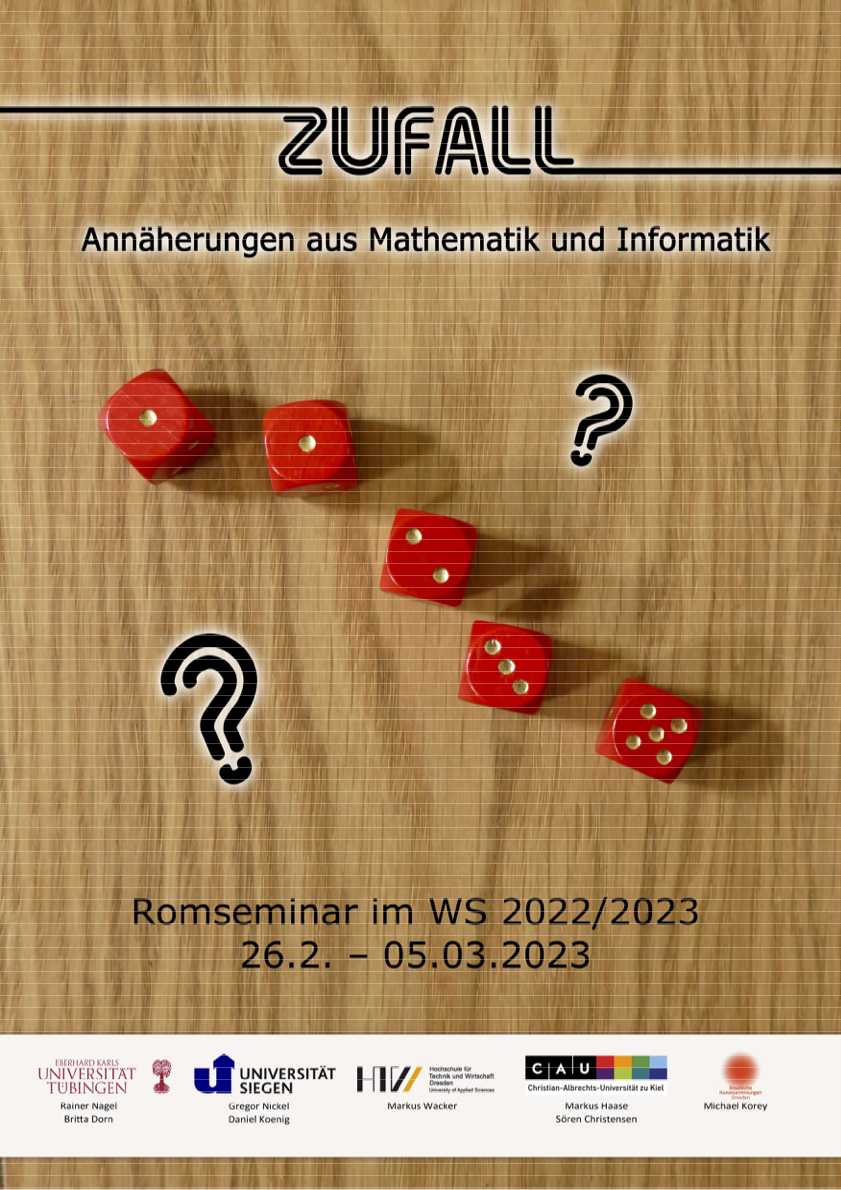
\includegraphics[width=14cm, height=12cm, keepaspectratio=true]{./content/Poster_Zufall}
	\vspace*{10pt}	  
	\end{center}
	%\end{flushright}
	\HRule
	\vspace*{\stretch{2}}
	\begin{center}
	  {Version: \today }
	\end{center}
\end{titlepage}

%\tableofcontents
%% !TEX root = ../Rom-Buch.tex
%% --
%% -- Rom-Vorwort.tex
%% --
\chapter*{Ein Vorwort}
\lipsum[1-2]
%% !TEX root = ../Rom-Buch.tex
%% --
%% -- Rom-Agenda.tex
%% -- ulgr: Besser mit lontable dieses machen
%% --
\chapter*{Die Agenda}
%% mit longtable setzen
Hier folgt die Agenda

\begin{description}
\item {\textbf{Sonntag, xx. März 2023}}
\begin{itemize}
\item[~] {Ankunft in Rom, Bezug der Unterkunft, Kennenlernen beim Pizzaessen: 
   Pizzeria ``Wanted'' an der Ecke Via Leonina Via dei Serpenti} (ca. 19 Uhr)
\end{itemize}
\smallskip

\end{description}

%\item {\textbf{Montag, 26. September 2022 -- Accademia dei Lincei}}
%\begin{itemize}
%\item[ 9$^{30}$] { Begr\"u{\ss}ung, Vorstellungsrunde}
%\item[10$^{30}$] {\textbf{Anastasia Boushmelev \& Lukas Strauch:}} {\emph{Die Große Vereinheitlichung.}}
%\item[12$^{00}$] {\textbf{Nina Henn:}} {\emph{Zur unverständlichen Effektivität der Mathematik.}}
%\item[13$^{00}$] \hfill {\textsc{Mittagspause}} \hfill ~
%\item[14$^{00}$] {\textbf{Aaron Kettner:}} {\emph{Die Jagd auf Schrödingers Katze: Lieber tot als lebendig?}}
%\item[15$^{00}$] {\textbf{Alice Maurer:}} {\emph{Replizierbarkeit -- das Problem aller empirischen Wissenschaften.}}
%\item[16$^{00}$] {\textbf{ Cornelia Vogel \& Michael Zimmermann:}} {\emph{Es werde Licht – Quantengravitation 
%  und andere philosophische Ansichten über die Entstehung der Welt.}}
%\item[18$^{30}$] \hfill {Cena (Pizzeria Da Baffetto, Via del Governo Vecchio 114, Roma)}  \hfill ~
%%   \hfill  {\footnotesize Treffpunkt: Piazza Navona am mittleren Brunnen}\hfill ~
%\end{itemize}
%\smallskip
%
%
%%\newpage
%
%
%\item {\textbf{Dienstag, 27. September 2022 -- Accademia dei Lincei / Villa del Priorato di Malta}}
%\begin{itemize}
%\item[9$^{15}$] {\textbf{Hannes Wagener:}} {\emph{Ökonomie jenseits von Mark und Plan?}}
%\item[10$^{15}$] {\textbf{Maximilian Weinberg:}} {\emph{Die `überforderte Gesellschaft'.}}
%\item[11$^{15}$] {\textbf{Tobias Bungart, Dennis Loch \& Jannik Marcel Nöll:}}  {\emph{Verschwörungstheorien.}}
%\item[12$^{45}$] \hfill {\textsc{Mittagspause}}\hfill ~
%%\newpage
%
%\item[15$^{00}$] {\textbf{Ivo Graziani (Chief of Cabinet of the Grand Hospitaller):}}
%         {\emph{Der Malteserorden und seine harten Probleme.}}
%\item[16$^{30}$] {Besichtigung der Magistralvilla und der Prioratskirche (Piranesi).}
%\end{itemize}
%\smallskip
%
%\newpage
%
%\item {\textbf{ Mittwoch, 28. September 2022 -- Bibliotheca Hertziana (MPI für Kunstgeschichte)}}
%\begin{itemize}
%\item[9$^{00}$] {\textbf{Dr. Sietske Fransen:}} {\emph{Von der Schwierigkeit, das Unbekannte zu visualisieren. 
%	Vorstellung eines Forschungsprojekts und Einführung in die Bibliotheca Hertziana.}}
%\item[9$^{30}$] \hfill {Kaffee-Empfang der Forschungsgruppe } ``Visualizing Science in Media Revolutions'' \hfill ~
%\item[10$^{15}$] {\textbf{Mohammad Yousuf Ejazi:}} {\emph{Härte-Maße in der Komplexitätstheorie.}}
%\item[11$^{15}$] {\textbf{Justus Springer:}} {\emph{Mathematik 4.0 – Die Automatisierung der Mathematik.}}
%\item[12$^{15}$] \hfill {\textsc{Mittagspause im Garten des Villino}} \hfill ~
%%{\bf :}  {\sl }
%%\item[14$^{0}$] {\bf :} {\sl }
%\item[14$^{00}$] {\textbf{M.A. Laura Valterio:}} {\emph{Die Bibliotheca Hertziana im Palazzo Zuccari.}}
%\item[15$^{00}$] {\textbf{Prof. Dr. Veronica Biermann:}} {\emph{Schwere Lasten in Rom. \\ Ein kunsthistorischer Rundgang.}}
%\item[20$^{00}$] \hfill {Vielleicht -- Viel-schwer. Eine literarische Soir\'ee (Hotel Tirreno)} \hfill ~
%%Besuch des Petrusgrabes und der Nekropole unter der Vatikanischen Basilika; alternativ:
%%\\\begin{footnotesize}Treffpunkt 14$^{00}$ am Petersdom bei der Schweizer Garde (links der Haupttreppe).\end{footnotesize}
%\end{itemize}
%%\smallskip
%
%
%\item {\textbf{Donnerstag, 29. September 2022 -- Villa Massimo (Deutschen Akademie Rom)}}
%\begin{itemize}
%\item[9$^{30}$]  {\textbf{Tobias Schnieders:}} {\emph{Wer von uns würde nicht gerne den Schleier lüften?}}
%\item[10$^{30}$] {\textbf{ Leon Duensing:}} {\emph{Es gibt ein Ignorabimus.}}
%\item[11$^{30}$] {\textbf{Dr. Julia Draganović:}} {\emph{Die Deutsche Akademie Rom -- Villa Massimo.}}
%\item[12$^{30}$] \hfill {\textsc{Mittagspause}} \hfill ~
%\item[13$^{30}$] {\textbf{Milan Bacchetta:}} {\emph{Über die schweren Probleme des Kletterns.}}
%\item[14$^{30}$] {\textbf{Prof. Dr. Veronica Biermann:}} {\emph{Kolossale Lasten heben oder \\ vom Gemachtsein 
%      der Architektur.}}
%\item[15$^{30}$] {Harte Probleme in der Kunst? -- Werkstattberichte nach Lust und Laune.} 
%\item[16$^{15}$] \hfill {\textsc{Musische Unterhaltung}} \hfill ~
%\end{itemize}
%%\smallskip
%\newpage
%
%\item {\textbf{Freitag, 30. September 2022 --  Genzano Palazzo Sforza-Cesarini / Lago di Nemi}}
%\begin{itemize}
%\item[9$^{00}$] {Abfahrt am Hotel Tirreno}
%\item[10$^{00}$] {\textbf{Prof. Dr. Rainer Nagel / Prof. Dr. Markus Haase:}}
%    {\emph{Lohnt die Beschäftigung mit schweren Problemen?}}
%\item[11$^{00}$] {\textbf{Jens Borgemeister:}} {\emph{Wissenschaft und Verantwortung.}}
%\item[12$^{00}$] {Abschlussgespr\"ach}
%\item[13$^{00}$] \hfill {\textsc{Imbiß auf der Terrasse des Palazzo}} \hfill ~
%\item[14$^{00}$] \hfill {Wanderung nach Nemi, Sentiero degli acquedotti} \hfill ~
%%\item[16$^{00}$] 
%\item[18$^{00}$] {Rückfahrt von Nemi nach Genzano}
%\item[19$^{00}$] \hfill {\textsc{Cena sociale (Genzano)}}  \hfill ~
%%{\footnotesize
%%Treffpunkt $^{?}$
%%}
%\end{itemize}
%%\smallskip
%
%
%%\newpage
%
%
%\item {\textbf{Samstag, 1. Oktober 2022 -- Alternative Besichtungen}}
%\begin{itemize}
%\item[11$^{45}$] {\textbf{Besichtigung:}}  {\emph{Domus Aurea}}	\\
%\item[15$^{00}$] {\textbf{Besichtigung:}}  {\emph{Case Romane}}	
%%{\sl Petersgrab}\\
%% {\footnotesize
%% Startpunkt: Obelisk am Petersplatz
%% }
%\end{itemize}
%%\smallskip
%
%
%\item {\textbf{Sonntag, 2. Oktober 2022}}
%\begin{itemize}
%\item[~] Abreise
%\end{itemize}
%%\smallskip
%
%
%\end{description}



%% -- Mainmatter
%% -- Beiträge der Teilnehmer
%% --

\mainmatter

% !TEX root = ../Rom-abcd.tex
%% -----------------------------------------------------
%% -- Musterdatei für die Erstellung des Beitrags
%% -- Stand: 2023/02/02
%% -----------------------------------------------------

%% -- Definitionen, damit die Eingabe einfacher wird
%% -- Bitte \renewcommand belassen
%% --
\renewcommand{\LongTitel}{Hier steht der lange Titel des Beitrags}
\renewcommand{\ShortTitel}{Hier steht der kurze Titel}
\renewcommand{\AutorenBeitrag}{Autor1, Autor2 \& Autor3}

%% -- Kapitelüberschrift und Eintrag in TOC
%% --
\addchap[\ShortTitel]{\LongTitel}
\addtocontents{toc}{\textsc{\AutorenBeitrag}}
\addtocontents{toc}{}

%% -- Kopfzeile 
%% -- Gerade Seiten : Autoren
%% -- Ungerade Seiten: Kurztitel
%% --
\markleft{\textsc{\AutorenBeitrag}}	
\markright{\textsc{\ShortTitel}}	

%% -- Titelseite des Beitrags
%% --
\begin{center}
\textsc{\Large \AutorenBeitrag}
\end{center}
	\vspace{1cm}
	
%% -- Bild der/des Vortragenden
\begin{center}
%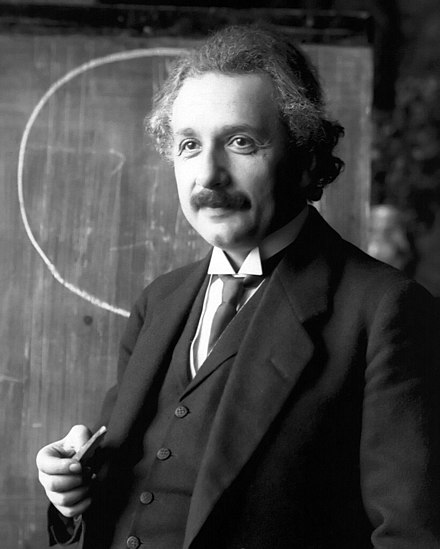
\includegraphics[width=8cm, height=8cm, keepaspectratio=true]{./content-abcd/autor1}
%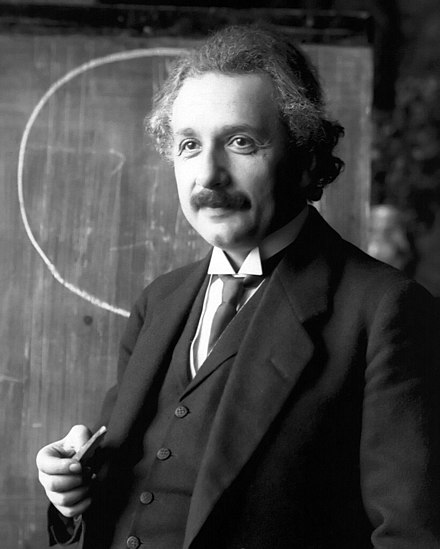
\includegraphics[width=8cm, height=8cm, keepaspectratio=true]{./content-abcd/autor1}
\end{center}

%% -- Die Referenzen werden am Ende des jeweiligen Beitrags ausgegeben
%% -- 
\begin{refsection}

%% -- Wer dies machen will
%% --
\dictum[\href{https://de.wikipedia.org/wiki/Albert_Einstein}{Albert Einstein}]{Wahnsinn ist, dasselbe immer \mbox{wieder} zu tun und andere Ergebnisse zu erwarten.}
%%
\begin{quote}
Für eine kurze Zusammenfassung
\end{quote}
%% 

%% --
\section*{Erster Hauptabschnitt}		%% 
\subsection*{Erster Unterabschnitt}		%% 
Text	
%%				
\subsection*{Zweiter Unterabschnitt}
Text
%% --
\section*{Zweiter Hauptabschnitt}		%% 
\subsection*{Erster Unterabschnitt}		%% 
%%
%% -- etc.
%% --

%% -- Literaturverzeichnis
%% --
\RaggedRight
\printbibliography
\end{refsection}


	
%% -- Backmattter
%% -- Literaturverzeichnis
%% -- Jeder Beitrag hat seine eigenes Literaturverzeichnis
%% --
%\backmatter
%\nocite{*}
%\printbibliography

%% --
\end{document} 